\section{eo\-Linear\-Truncate$<$ EOT $>$ Class Template Reference}
\label{classeo_linear_truncate}\index{eoLinearTruncate@{eoLinearTruncate}}
a truncate class that does not sort, but repeatidely kills the worse.  


{\tt \#include $<$eo\-Reduce.h$>$}

Inheritance diagram for eo\-Linear\-Truncate$<$ EOT $>$::\begin{figure}[H]
\begin{center}
\leavevmode
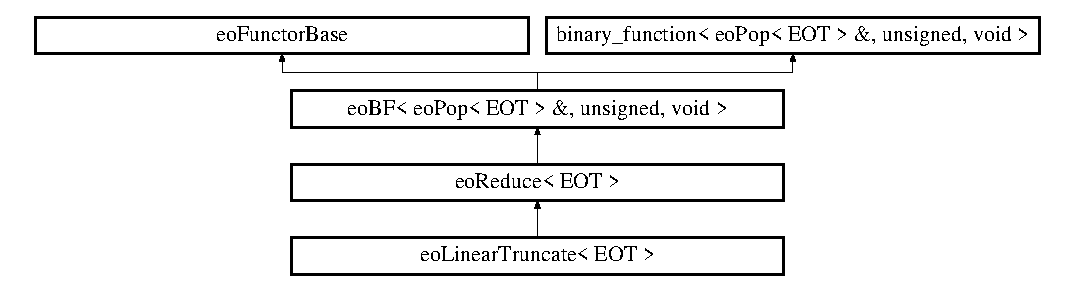
\includegraphics[height=3.45679cm]{classeo_linear_truncate}
\end{center}
\end{figure}
\subsection*{Private Member Functions}
\begin{CompactItemize}
\item 
void {\bf operator()} ({\bf eo\-Pop}$<$ {\bf EOT} $>$ \&\_\-newgen, unsigned \_\-newsize)\label{classeo_linear_truncate_d0}

\begin{CompactList}\small\item\em The pure virtual function that needs to be implemented by the subclass. \item\end{CompactList}\end{CompactItemize}


\subsection{Detailed Description}
\subsubsection*{template$<$class EOT$>$ class eo\-Linear\-Truncate$<$ EOT $>$}

a truncate class that does not sort, but repeatidely kills the worse. 

To be used in SSGA-like replacements (e.g. see {\bf eo\-SSGAWorse\-Replacement}{\rm (p.\,\pageref{classeo_s_s_g_a_worse_replacement})}) 



Definition at line 167 of file eo\-Reduce.h.

The documentation for this class was generated from the following file:\begin{CompactItemize}
\item 
eo\-Reduce.h\end{CompactItemize}
